\chapter{Analyse de malwares}
\section{Introduction}
L'analyse de malwares (malware analysis) est aujourd’hui devenue une activité très importante dans le cadre de la gestion des incidents de sécurité informatique. Les organisations qui prennent sérieusement en compte la sécurité de leurs réseaux sont souvent confrontées a des fichiers suspects capturés grâce à leurs antivirus, IDS et systèmes de supervision sécurité, ou encore lors d'analyses forensics. Il est alors nécessaire d'analyser rapidement ces fichiers pour déterminer s'il s'agit de code malveillant connu, d'une attaque ciblée ou bien d'un faux positif. Connaître le comportement d'un malware est capital pour déterminer si d'autres machines sur le réseau peuvent être compromises ou non, et pour décider comment réagir.\\


L'analyse statique de code exécutable par désassemblage a beaucoup de succès et permet d'obtenir d'excellents résultats, cependant la complexité de ce processus demande un long apprentissage, beaucoup de temps et d'énergie. De plus il n'est pas rare de rencontrer des codes malveillants protégés contre le désassemblage et le débogage, ce qui peut ralentir considérablement l'analyse.\\


L'analyse dynamique de code malveillant est une autre méthode qui consiste à faire exécuter un échantillon de code sur une plate-forme conçue pour observer toutes ses actions. Dans la plupart des cas, c'est une approche très efficace et rapide pour déterminer la nature et le comportement du code malveillant, au moins dans un premier temps.

\section{Objectifs de l'analyse de malwares}
Voici quelques-uns des objectifs habituels d'une analyse de malware :\\


\begin{itemize}
\item Vérifier si un fichier suspect est effectivement malveillant ou s'il s'agit d'un faux positif
\item Déterminer s'il s'agit d'un code malveillant générique (connu ou non) ou bien d'une attaque ciblée
\item Obtenir des informations sur la source de l'attaque
\item Déterminer toutes les actions du code malveillant sur le système local : fichiers créés/modifiés/supprimés, processus lancés/stoppés, clés de registre, services installés, ...
\item Déterminer toutes ses actions sur le réseau : connexions sortantes, réplication, serveur en écoute, ...
\item Déterminer ses "fonctionnalités" malveillantes : virus, ver, cheval de Troie, porte dérobée, bombe logique, rootkit, keylogger, téléchargement, relais de spam, déni de service, botnet, ...
\item Déterminer quelles sont les machines ciblées et lesquelles pourraient être vulnérables ou déjà compromises sur le réseau
\item Fournir des informations pour mieux cibler une éventuelle analyse forensics d'autres machines (noms de processus, empreintes MD5 de fichiers, clés de registre, mots clés, ...)
\item Décider quelles actions entreprendre pour gérer l'incident
\item Comprendre comment la compromission s'est déroulée afin d'améliorer les protections à l'avenir.\\
\end{itemize}

\section{Où trouver des malwares ?}

Il existe toute une communauté autour de l'analyse de malwares : forums, sites, blogs, etc. Certains de ces sites mettent à disposition des échantillons permettant d'effectuer des analyses. Quelques adresses :
\begin{list}{•}{}
\item \textbf{KernelMode : }Forum d’échange et d’analyse de malwares. Met à disposition des lecteurs des échantillons~\cite{mal1} 
\item  \textbf{Malware.lu : }Excellent site mettant à disposition des échantillons de malwares et proposant des analyses~\cite{mal2}
\item \textbf{Contagio Exchange : }Site permettant d'échanger et de télécharger des malwares~\cite{mal3}
\item \textbf{CrowdRE : }Plate-forme collaborative d'analyse de malwares~\cite{mal4}
\item \textbf{VadeRetro Sales malwares : }Articles et tutoriaux sur les malwares~\cite{mal5}
\item \textbf{Malekal's Site : }Excellent site consacré à l'entraide informatique. De nombreux exemples d'analyses comportementales~\cite{mal6}
\item \textbf{Malware Analysis \& Diagnostics : }Analyse de malwares~\cite{mal7} 
\item \textbf{FireEye Malware Intelligence Lab : }Site de recherche et d'analyses de malwares~\cite{mal8}
\item \textbf{Evil3ad : }Site d'analyse de malwares~\cite{mal9}
\item \textbf{M86SecurityLabs : }Site consacré aux attaques (malwares, cybercriminalité)~\cite{mal10}
\item \textbf{Fun in malwares analysis :} Tutoriaux sur l'analyse de malwares~\cite{mal11}.\\
\end{list}



Les blogs des compagnies antivirales publient aussi de nombreuses analyses :
\begin{list}{•}{}
\item \textbf{Blog de Kaspersky : }~\cite{blog1}
\item \textbf{Blog d'Eset : }~\cite{blog2} 
\item \textbf{Blog de Norton : }~\cite{blog3}
\item \textbf{Blog de Sophos : }~\cite{blog4}.\\
\end{list}
\section{Construire un laboratoire sécurisé d'analyse de malwares}

Dans la section précédente, nous avons vu différentes méthodes pour récupérer des malwares. Maintenant comment les étudier en toute sécurité ? Il est bien sûr "impensable" de les exécuter et de les analyser sur un poste de travail. Il convient donc de créer un environnement spécial permettant de les analyser en toute sécurité.
\subsection{La virtualisation}
La virtualisation a révolutionné de nombreux domaines de l’informatique dont le domaine de l’analyse des malwares. Il devient ainsi simple et rapide de tester des malwares dans des environnements contrôlés afin de découvrir leurs actions.\\

Parmi les outils les plus utilisés dans le domaine de la virtualisation personnelle, nous pouvons citer principalement \textbf{Vmware}~\cite{vm}(payant) ainsi que \textbf{VirtualBox}~\cite{vbox} (gratuit). Par contre certains malwares possèdent des fonctionnalités de détection d'environnements virtuels et stoppent leur exécution.
\subsubsection{Avantages de la virtualisation}
\begin{itemize}
\item \textbf{Coût et flexibilité :} une seule machine physique permet de simuler deux machines ou plus, et de construire différentes
architectures réseau suivant les besoins.
\item \textbf{Sécurité :} les machines virtuelles peuvent être connectées par un réseau virtuel totalement indépendant de tout réseau
opérationnel, sans risque d'infecter d'autres machines.
\item \textbf{Rapidité et efficacité :} une machine virtuelle peut être stoppée, restaurée et redémarrée en quelques secondes.
\item \textbf{Facilité d'emploi :} n'importe quel état de fonctionnement peut être sauvegardé dans un "snapshot" en quelques secondes. Il est ensuite très simple de restaurer tout snapshot précédent, et de comparer plusieurs états entre eux.
\item Les machines virtuelles peuvent être facilement copiées, dupliquées et modifiées pour constituer une bibliothèque de toutes les versions d’un système d’exploitation ou d’une application.
\end{itemize}
\subsubsection{Inconvénients de la virtualisation}
\begin{itemize}
\item Il existe de nombreuses techniques connues utilisables par des malwares pour détecter s'il s'exécutent dans une machine virtuelle. Dans ce cas ils peuvent éviter de s'exécuter ou perturber l'analyse.
\item Certains environnements de virtualisation peuvent être vulnérables et permettre à un code malveillant spécifiquement conçu de "s'échapper" d'une machine virtuelle pour compromettre le système hôte. Il est donc utile de prendre quelques précautions
lors de toute exécution de code malveillant.
\end{itemize}


\subsection{Considérations du système d'exploitation}
Les malwares comportent radicalement différent selon le système d'exploitation lequel sont exécutés sur. Certains malwares ne peuvent fonctionner que sur les systèmes d'exploitation Microsoft Windows Server, tandis que d'autres programmes malveillants ne peuvent fonctionner que sur des versions spécifiques du noyau Linux. Malware qui est installé sur un hôte Microsoft Windows Vista peut crasher complètement le système, tandis que le même malware installé sur un système Microsoft Windows 7 pourrait rejoindre un réseau de zombies (botnet). C'est une nécessité d'avoir une variété de systèmes d'exploitation disponibles lors de l'analyse des programmes malveillants. Donc il faut avoir différents systèmes d'exploitation comme Microsoft Windows XP, Microsoft Windows 7, Microsoft Windows Server 2003, et l'une des distributions Linux les plus populaires modernes comme Ubuntu pour servir d'hôtes infectés.
\subsection{L'isolement du réseau}
Des précautions supplémentaires doivent être prises en ce qui concerne l'emplacement des hôtes d'analyse des malwares sur le réseau. Les vers (Worms) et autres types de programmes malveillants peuvent avoire la fonction "auto-réplication", il est donc très probable que l'exécution de malware sur une machine du réseau peut conduire à d'autres hôtes sur ce réseau.\\
Un argument supplémentaire pour isoler les machines de laboratoire de l'Internet est d'empêcher les auteurs des logiciels malveillants de savoir l'existence de l'analyste. Il est tout à fait probable que le malware exécuté est configuré pour "phone home" à une commande \& contrôle le serveur qui permet à l'auteur de savoir  que vous avez exécuté le malware. À ce stade, l'attaquant pourrait commencer l'exécution de commandes sur le système de laboratoire pour tenter de désactiver ou déjouer les tentatives d'analyse.\\

La figure~\ref{fig :lab} donne un exemple de laboratoire d'analyse de malwares.
\begin{figure}[H]
\begin{center}
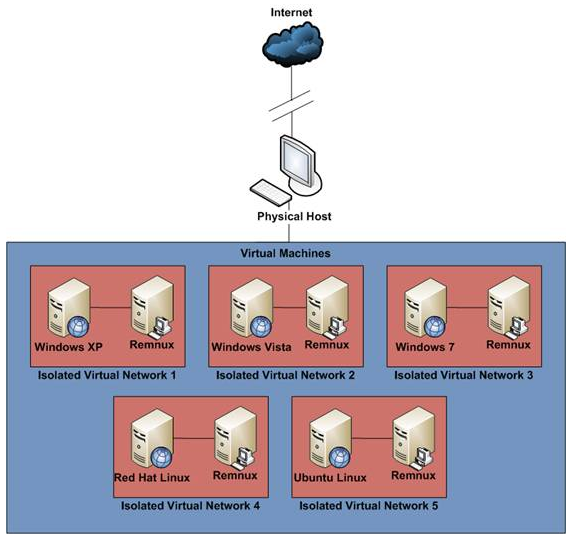
\includegraphics[scale=0.65]{Figures/lab.png}
\caption{Exemple d'un laboratoire d'analyse de malwares.}
\label{fig :lab} 
\end{center}
\end{figure}

\subsection{Les distributions dédiées à l'analyse de malwares}


Il existe des distributions consacrées spécialement à l'analyse de malwares, une d'elle est particulièrement connue : \textbf{REMnux}(Figure~\ref{fig :rem}). C'est une distribution Ubuntu conçue spécialement pour l'analyse de malwares. Elle contient des outils pour analyser la mémoire, des documents pdf vérolés, le réseau, ...\\
\begin{figure}[H]
\begin{center}
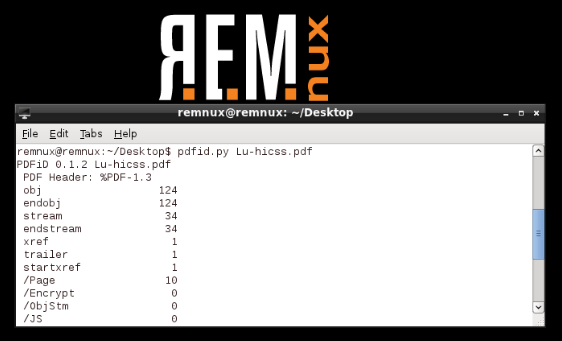
\includegraphics[scale=0.5]{Figures/remnux.png}
\caption{Remnux, distribution pour l'analyse de malwares.}
\label{fig :rem} 
\end{center}
\end{figure}


Il existe aussi une distribution nommée \textbf{Zero Wine}(Figure~\ref{fig :wine}) qui permet d'analyser le comportement d'un malware : le malware est exécuté dans un bac à sable (sandbox) puis de nombreux rapports sont générés.
\begin{figure}[H]
\begin{center}
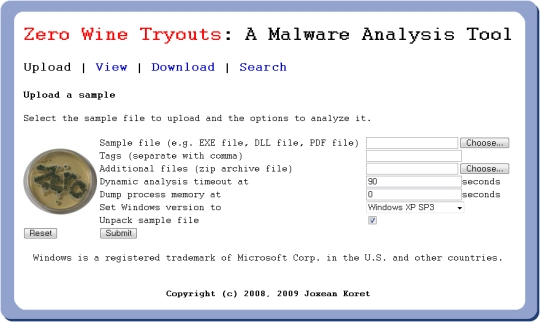
\includegraphics[scale=0.7]{Figures/wine.jpg}
\caption{Distribution ZeroWine pour l'analyse de malwares.}
\label{fig :wine} 
\end{center}
\end{figure}
\section{Les méthodologies d'analyse de malwares}
\subsection{L'analyse statique}
\subsubsection{Définition}
L'analyse statique de malwares consiste à explorer le contenu des fichiers suspects à l'aide de divers outils, dans le but d'extraire le maximum d'informations sans exécuter le code malveillant qu'ils pourraient contenir. A ce stade il s'agit uniquement
d'observer le contenu "visible". Le premier outil à employer dans ce cas est
toujours un afficheur texte/hexadécimal.\\

Une analyse directe de ce type permet souvent de révéler beaucoup d'informations utiles grâce aux chaînes de caractères qui apparaissent en clair, aux entêtes de fichiers, aux méta-données, etc. Il est même parfois possible d'extraire des données camouflées par des méthodes simples (i.e. "XOR"), sans recourir à des méthodes d'analyse sophistiquées. Dans le cas de document malformés (par exemple des exploits pour MS Office, PDF, ...), des outils de "file carving" peuvent souvent extraire les fichiers exécutables malveillants stockés à l'intérieur.\\

Voici le type d'informations utiles qu'il est souvent possible d'extraire :\\
\begin{itemize}


\item Types de fichiers
\item Présence de code malveillant connu ou non
\item Adresses IP, URLs, noms de domaines ou de machines (cibles du code malveillant, serveur de téléchargement ou bien connexion retour vers un serveur de contrôle)
\item Date de création des fichiers, auteur, organisation et autres informations (méta-données dans les documents)
\item Encodages utilisés (qui peuvent trahir une provenance exotique)
\item Présence possible de shellcodes ("NOP sleds" : typiquement une longue suite d'octets 0x90)
\item Mots clés particuliers qui peuvent indiquer une attaque ciblée : nom de l'entreprise, noms de serveurs, d'applications ou d'utilisateurs spécifiques, mots de passe internes, etc.

\end{itemize}
\subsubsection{Le désassemblage}
Le désassemblage (reverse engineering) consiste à ouvrir un fichier exécutable avec des outils tel que \textbf{IDA pro}, ou \textbf{Metasm} par exemple afin de retrouver et d'analyser le code assembleur correspondant au contenu binaire du fichier. Certains outils avancés peuvent même offrir des fonctions de décompilation permettant de reconstruire le code source de haut niveau employé au départ (en général C).\\
En analysant le code, il est ainsi possible d'étudier le comportement de chaque partie du programme et d'en déduire les fonctionnalités.\\

L'avantage de cette méthode est qu'en théorie il est possible d'analyser tout le code, même celui ne s'exécutant que sous certaines conditions particulières. De nombreux malwares ont par exemple des fonctions pour ne pas s'exécuter dans un environnement virtuel, ce qui empêche une analyse dynamique. Dans ce cas, seul le désassemblage peut permettre l'analyse du malware. Il est aussi possible de trouver d'éventuelles routines d'obfuscations employées afin de masquer les données sensibles du code malveillant (mot de passe, clés de chiffrement, adresse des serveurs, etc.)\\

Cependant le désassemblage a quelques inconvénients :\\

\begin{itemize}
\item Il  \textbf{nécessite de grandes compétences} afin de pouvoir lire et d'analyser du code assembleur. Il faut connaître les correspondances systèmes entre le code, les langages de haut niveau et les appels systèmes
\item \textbf{L'analyse complète d'un fichier peut représenter beaucoup de temps} (de plusieurs jours à plusieurs semaines), de compétences et d'énergie selon la taille et la complexité du code
\item \textbf{Certains malwares sont protégés contre le désassemblage} à l'aide de techniques de compression et de chiffrement. Ces protections, jamais parfaites, peuvent néanmoins ralentir l'analyse et demander beaucoup d'efforts pour être cassées.
\end{itemize}
\subsubsection{Les outils et les services d'analyse statique}
\begin{itemize}
\item \textbf{La commande file : }file est une commande d'UNIX qui permet de déterminer le type d'un fichier.\\
Pour chaque fichier valide passé en paramètre, file tente de déterminer le type de données qu'il contient et affiche cette information et éventuellement d'autres informations comme les dimensions pour une image ou les codecs.\\
La figure~\ref{fig :file} donne un exemple d'utilisation de la commande file :
\begin{figure}[H]
\begin{center}
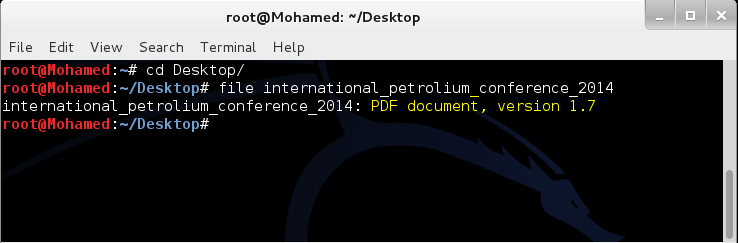
\includegraphics[scale=0.7]{Figures/file.png}
\caption{Utilisation de la commande file.}
\label{fig :file} 
\end{center}
\end{figure}
\item L'outil \textbf{md5sum : }est un utilitaire en ligne de commande qui permet de vérifier l'intégrité d'un fichier. En effet, il permet de récupérer et comparer des empreintes MD5 des fichiers.\\
La figure~\ref{fig :md5} donne un exemple d'utilisation de l'outil md5sum :
\begin{figure}[H]
\begin{center}
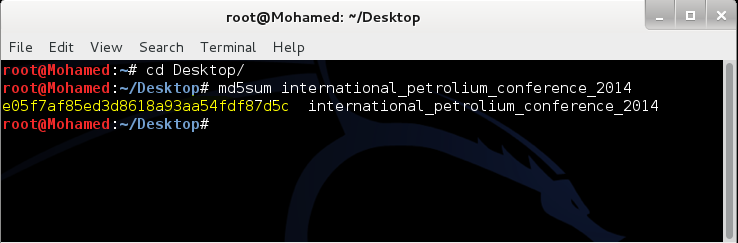
\includegraphics[scale=0.7]{Figures/md5sum.png}
\caption{L'outil md5sum.}
\label{fig :md5} 
\end{center}
\end{figure}
\item \textbf{Antivirus scaninig :}Après la récupération de hash md5 de malware qui va nous permettre de savoir si ce malware a été déjà analysé par une autre personne. Pour ce
faire, on peut trouver des sites qui permettent d'accomplir cette tâche. Il suffit d'entrer le fichier et il va vérifier s'il s'agit d'un malware connu ou non. On peut citer comme exemple le site suivant \url{www.virustotal.com} qui permet d'analyser le fichier avec 52 antivirus différents. Cette étape est très importante dans le but de ne pas perdre du temps dans l'analyse d'un malware déjà connu.\\
La figure montre la page web VirusTotal.com :
\begin{figure}[H]
\begin{center}
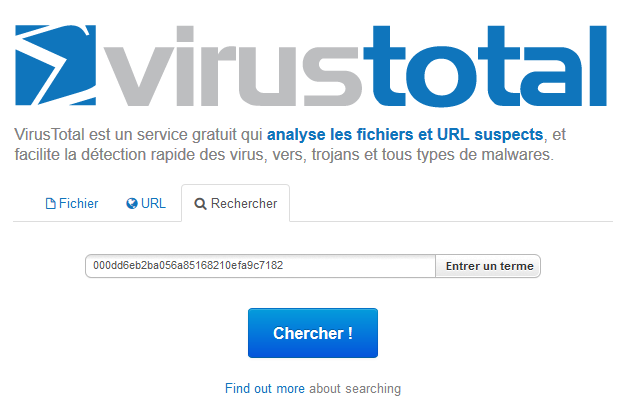
\includegraphics[scale=0.5]{Figures/vit.png}
\caption{Aperçu sur l'interface du site www.virustotal.com.}
\label{fig :vit} 
\end{center}
\end{figure}
\item \textbf{Strings de Sysinternals suite : }Recherche pour ANSI et UNICODE chaînes dans les fichiers.\\
La figure~\ref{fig :strings} montre un exemple d'utilisation de l'outil strings :
\begin{figure}[H]
\begin{center}
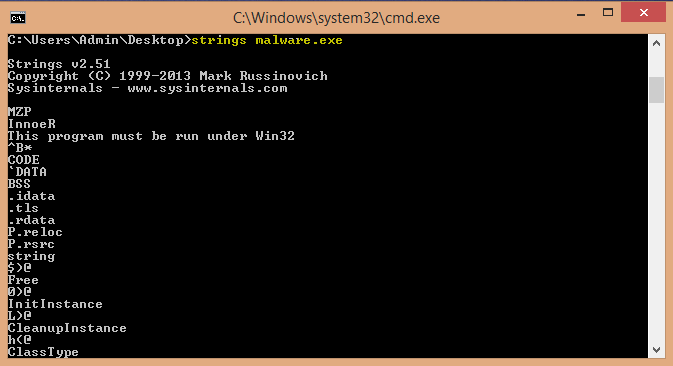
\includegraphics[scale=0.7]{Figures/strings.png}
\caption{L'outil strings de Sysinternals suite.}
\label{fig :strings} 
\end{center}
\end{figure}
\item \textbf{PEiD : }Il détecte les packers et les compilateurs les plus courants pour les fichiers PE. Il est actuellement possible de détecter plus de 470 signatures différentes dans les fichiers portable exécutable.\\
La figure~\ref{fig :pei} montre le programme PEiD.
 \begin{figure}[H]
\begin{center}
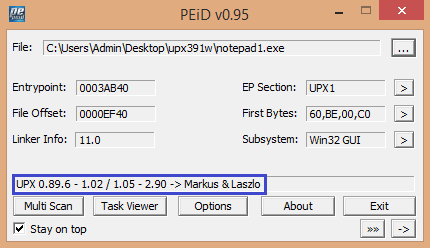
\includegraphics[scale=0.8]{Figures/PEID.png}
\caption{L'interface de PEiD.}
\label{fig :pei} 
\end{center}
\end{figure}
\item \textbf{Les désassembleurs : }Parmi les outils les plus connus pour le désassemblage, il y a bien sûr \textbf{IDA}. IDA  est un désassembleur commercial très utilisé en rétro-ingénierie. Il supporte une grande variété de formats exécutables pour différents processeurs et systèmes d'exploitation.\\
IDA permet de passer du code binaire du malware vers son code assembleur. De plus, on peut lui ajouter le plugin Hex-Ray qui va nous permettre de faire la décompilation (c'est-à-dire revenir au code C).\\
La figure~\ref{fig :ida} montre le programme IDA :
\begin{figure}[H]
\begin{center}
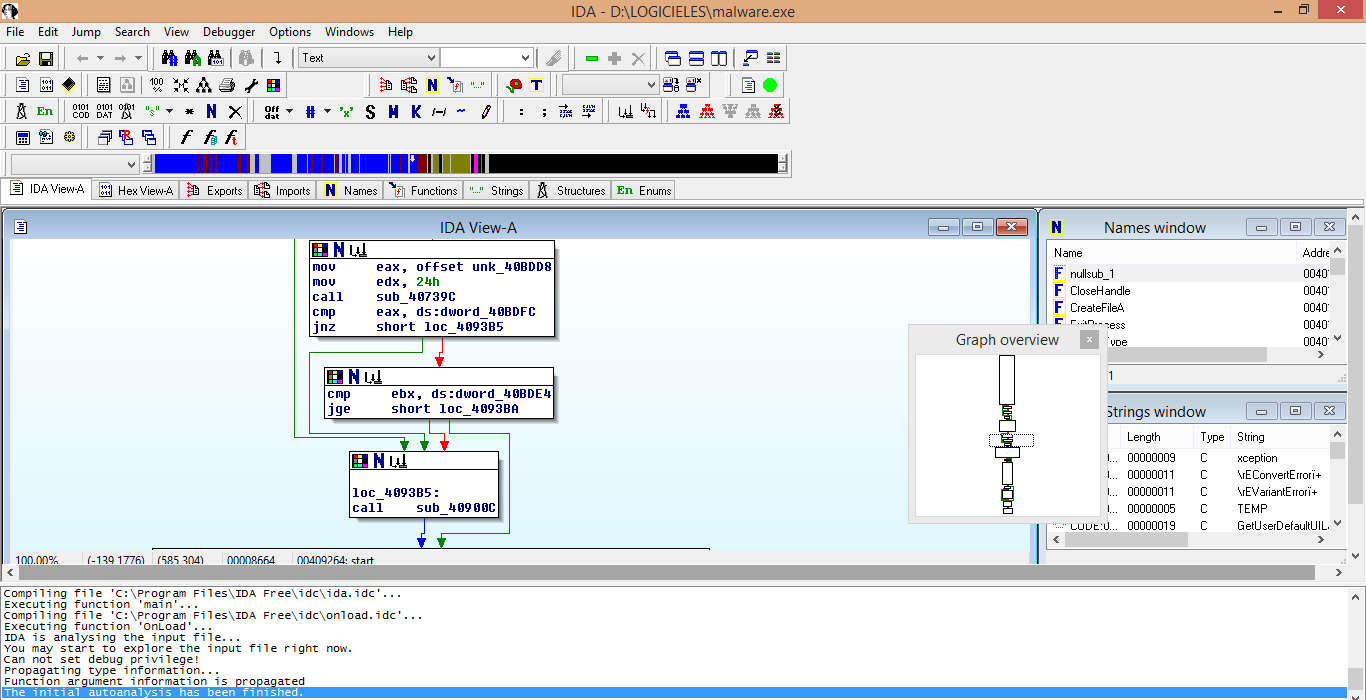
\includegraphics[scale=0.42]{Figures/ida.png}
\caption{Interface d'IDA Pro Free.}
\label{fig :ida} 
\end{center}
\end{figure}
\end{itemize}
\subsection{L'analyse dynamique}
\subsubsection{Définition}
Contrairement à l'analyse statiques, l'analyse dynamique consiste à exécuter réellement le code malveillant dans un environnement adéquat afin d'observer toutes ses actions et d'en déduire son comportement global. Ce type de méthode est parfois appelée analyse comportementale.\\


Cette méthode apporte plusieurs avantages par rapport au désassemblage statique :
\begin{itemize}
\item Elle est beaucoup plus rapide. En quelques minutes, il est déjà possible d'avoir un aperçu des principales fonctionnalités du malware
\item Elle ne nécessite pas de connaissances en assembleur ou en programmation.
\item Elle n'est pas sensible aux techniques de protection des malwares (obfuscation, anti-désassemblage, etc).\\
\end{itemize}

Par contre, l'analyse comportementale n'est pas efficace dans certains cas :
\begin{itemize}

\item Si certaines fonctionnalités du malware nécessitent des conditions particulières pour être exécutées, elles peuvent ne pas être détectées lors de l'analyse
\item Certains malwares contiennent des fonctionnalités permettant de détecter qu'ils sont dans un environnement contrôlé et de ne pas s'exécuter dans ces cas là
\item L'analyse comportementale ne permet pas toujours d'accéder aux informations sensibles contenues dans le malware.
\end{itemize}
\subsubsection{Les outils d'analyse dynamique}
\begin{itemize}
\item \textbf{Process Monitor et Capture BAT : }Permettent de surveiller l'activité du système de fichiers, du Registre, des processus, des thread et des DLL en temps réel.. Ces outils peuvent aider à comprendre comment les tentatives de logiciels malveillants à intégrer dans le système lors de l'infection.\\
La figure~\ref{fig :procmon} montre l'interface de programme Process Monitor :
\begin{figure}[H]
\begin{center}
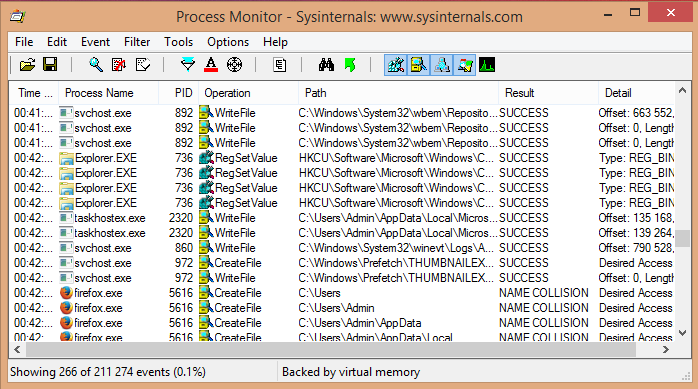
\includegraphics[scale=0.7]{Figures/procmon.png}
\caption{L'outil Process Monitor de Sysinternals suite.}
\label{fig :procmon} 
\end{center}
\end{figure}
\item \textbf{ Process Explorer et Process Hacker : }Iles indiquent quels fichiers ont été ouverts par les clés de registre et autres processus d'objet, quelles DLL ils ont chargées, le propriétaire de chaque processus, et bien plus encore.  \\
La figure~\ref{fig :proexp} montre l'utilitaire Process Explorer :
\begin{figure}[H]
\begin{center}
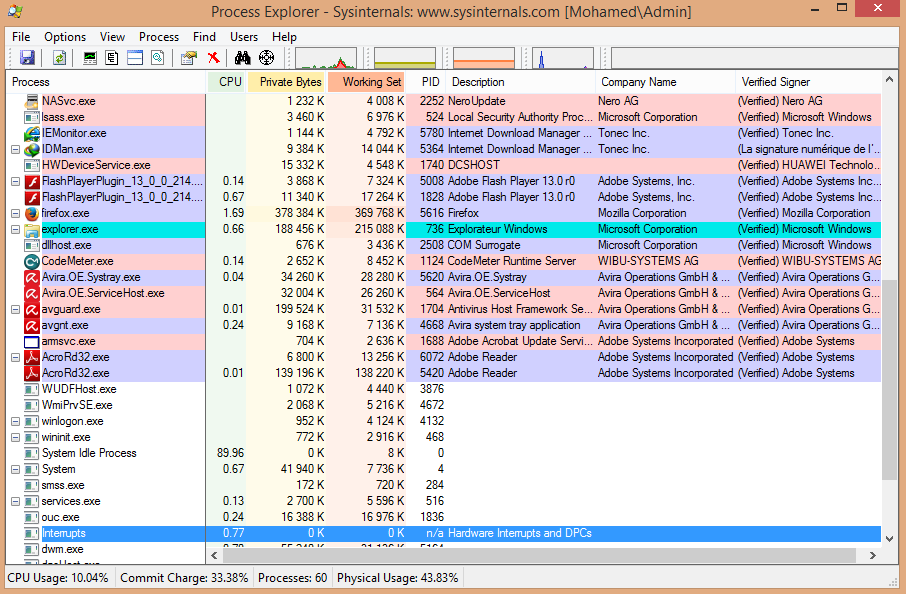
\includegraphics[scale=0.6]{Figures/procexp.png}
\caption{L'outil Process Explorer de Sysinternals suite.}
\label{fig :proexp} 
\end{center}
\end{figure}
\item \textbf{Wireshark et SmartSniff : }Ils sont des analyseurs réseau, qui peuvent capturer le trafic réseau de laboratoire pour les tentatives de communication malveillants, tels que les demandes de résolution de DNS, le trafic de bot, ou des téléchargements.\\

La figure~\ref{fig :wire} montre l'interface ce Wireshark :
\begin{figure}[H]
\begin{center}
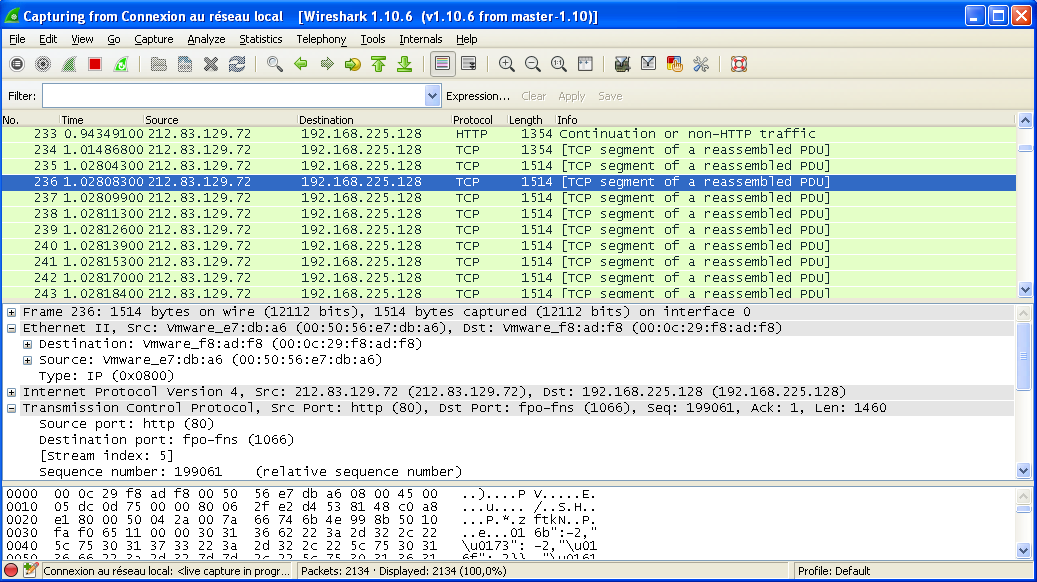
\includegraphics[scale=0.55]{Figures/wire.png}
\caption{L'interface de Wireshark.}
\label{fig :wire} 
\end{center}
\end{figure}
\item \textbf{Regshot : }Est est un outil léger pour comparer l'état du système avant et après l'infection, de mettre en évidence les principaux changements  apportées par le malware au système de fichiers et les Registres.\\

La figure montre le programme Regshot :
\begin{figure}[H]
\begin{center}
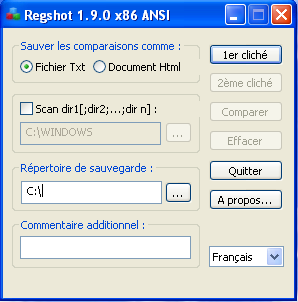
\includegraphics[scale=0.85]{Figures/reg.png}
\caption{L'interface de Regshot.}
\label{fig :reg} 
\end{center}
\end{figure}
\item \textbf{Cuckoo Sandbox : }Ce bac à sable (sandbox) permet en quelques minutes d'obtenir une première estimation des capacités d'un malware et de ses communications avec l'extérieur ou encore de connaître les fichiers crées sur le système. Gratuit, il nécessite d'être installé sur une station hôte saine et de lui soumettre des malwares qui seront analysés de façon totalement automatisée dans une machine virtuelle.\\

La figure~\ref{fig :cuckoo} montre l'interface Cuckoo Sandbox :
\begin{figure}[H]
\begin{center}
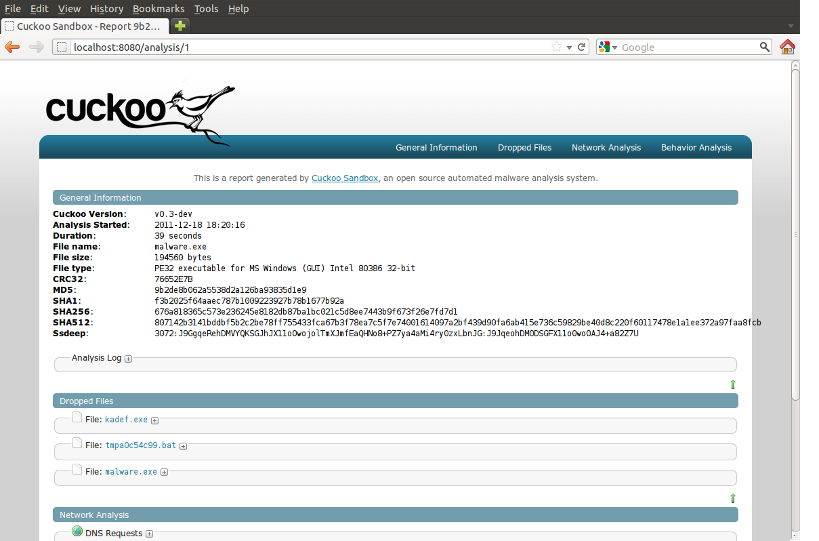
\includegraphics[scale=0.7]{Figures/cuckoo.png}
\caption{L'interface de Cuckoo Sandbox.}
\label{fig :cuckoo} 
\end{center}
\end{figure}
Par rapport à d'autres services en ligne de ce type, Cuckoo permet d'analyser très rapidement en première approche des binaires ou documents suspects dans un environnement sécurisé tout en gardant la confidentialité des données ce que ne permettent pas les services de ligne.
\end{itemize}
\subsection{L'analyse des documents malveillants}
Les documents malicieux se sont énormément développés ces dernières années et constituent un vecteur d'attaque très utilisé par les malwares. Nous nous focaliserons ici sur les documents de la famille Microsoft Office et les documents PDF, ceux-ci pouvant se révéler très complexes. Du point de vue de l'analyste, la problématique qui se pose est de savoir si le document à analyser possède une charge malicieuse. La génération de documents malicieux est très simple et nombreux sont les outils d'intrusion qui possède de telles fonctionnalités.
\subsubsection{L'analyse des documents PDF malveillants}

Depuis l'année 2009, les attaques au moyen de fichiers PDF (Portable Document Format) malveillants se sont multipliées. Par exemple :\\

\begin{itemize}


\item Pour l'année 2009 le Cert-IST a émis 4 Dangers Potentiels pour avertir notre communauté de nouvelles attaques utilisant des vulnérabilités dans Adobe Reader ou dans Adobe Acrobat
\item L'éditeur antivirus BitDefender a placé en tête de son "Top 10 pour décembre 2009" la menace "Exploit.PDF-JS.Gen" qui représente 12,04\% de l'ensemble des infections. Sous ce nom sont regroupés des fichiers PDF qui exploitent différentes vulnérabilités détectées dans le moteur JavaScript de PDF Reader, afin d'exécuter du code malveillant sur l'ordinateur de l'utilisateur~\cite{PDF}.
\end{itemize}
\subsubsection*{Les outils d'analyse des documents PDF malveillants}
\begin{itemize}
\item \textbf{pdfid : }identifie les fichiers PDF qui contiennent des chaînes associées à son exécution des scripts et des actions
\item \textbf{pdf-parser : }examine la structure de fichiers PDF
\item \textbf{PDF Stream Dumper : }combine de nombreux outils d'analyse de fichiers PDF sous une interface graphique
\item \textbf{peepdf : }
offre un shell interactif en ligne de commande pour examiner les fichiers PDF.
\end{itemize}
\section{Partie pratique}
\subsection{Présentation du malware}
Le PDG d'une entreprise pétrolière a reçu un mail contenant un document PDF en rapport avec une conférence internationale.\\
Une fois le PDF ouvert, il s'est rendu compte que le fichier ne correspondait pas à la conférence et que c'était seulement un brouillon de document. Il a alors décidé de l'envoyer à son RSSI (Responsable de Sécurité des Systèmes Informatiques) pour vérifier si 
le document n'est pas malicieux.
\subsection{L'analyse statique}
\subsubsection*{Étape 1 : Type de fichier}
On ouvrant le document suspect avec un éditeur hexadécimal, on voit dans la figure~\ref{fig :anal1} qu'il est bien un document PDF version 1.7.
\begin{figure}[H]
\begin{center}
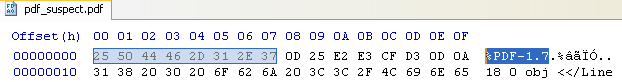
\includegraphics[scale=0.7]{Figures/anal1.png}
\caption{Vérification de type de fichier dans l'éditeur HxD.}
\label{fig :anal1} 
\end{center}
\end{figure}
\subsubsection*{Étape 2 : Récupérer le hash MD5 de fichier}
On utilisant l'application "WinMD5" pour récupérer le hash MD5 de document PDF, la figure~\ref{fig :anal2} montre le hash du fichier.
\begin{figure}[H]
\begin{center}
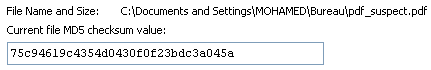
\includegraphics[scale=1]{Figures/anal2.png}
\caption{Le hash MD5 de fichier avec "WinMD5".}
\label{fig :anal2} 
\end{center}
\end{figure}
\subsubsection*{Étape 3 : Antivirus scanning}
Après avoir récupérer le hash MD5 de document PDF, qui va nous permettre de savoir si ce malware a été déjà analysé par une autre personne. On utilisant "virustotal", on voit dans la figure que le document PDF n'a pas été analysé auparavant.
\begin{figure}[H]
\begin{center}
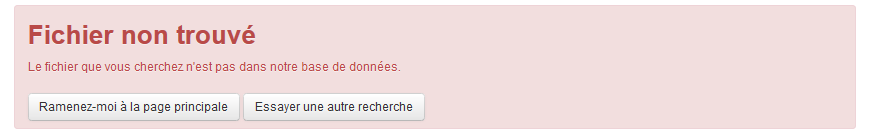
\includegraphics[scale=0.7]{Figures/anal3.png}
\caption{Le scan avec VirusTotal.}
\label{fig :anal3} 
\end{center}
\end{figure}
\subsubsection*{Étape 4 : pdfid et pdf-parser}
Pdfid identifie les fichiers PDF qui contiennent des chaînes associées à son exécution des scripts et des actions, la figure~\ref{fig :anal4} montre que ce document PDF contient un "javasript" et "Automatic Action" donc on peut dire que le document est malveillant.\\
Ce document PDF contient un contenu Flash. Très souvent, les attaquants utilisent Flash intégré afin d'essayer d'exploiter le flash Adoble et exécuter du code arbitraire ou de provoquer un déni de service lors de l'ouverture d'un document PDF malveillant.
\begin{figure}[H]
\begin{center}
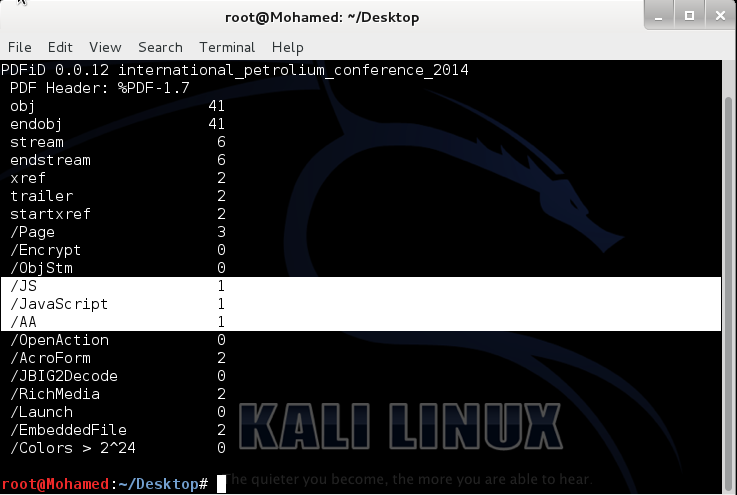
\includegraphics[scale=0.5]{Figures/anal4.png}
\caption{L'interface de PDFiD.}
\label{fig :anal4} 
\end{center}
\end{figure}
Avec pdf-parser, on voit dans la figure~\ref{fig :anal5} le code javascript :

\begin{figure}[H]
\begin{center}
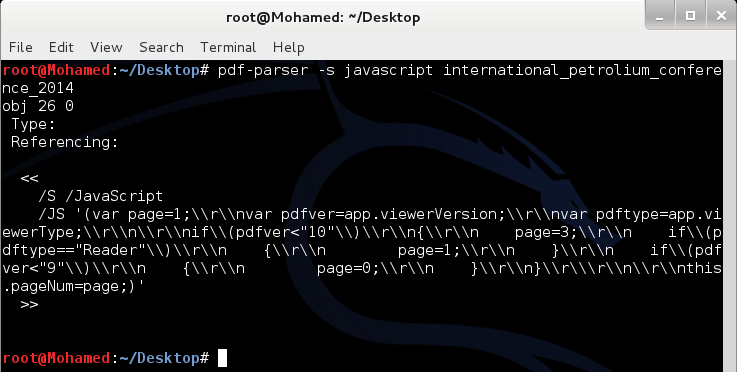
\includegraphics[scale=0.6]{Figures/anal5.png}
\caption{L'interface de paf-parser.}
\label{fig :anal5} 
\end{center}
\end{figure}
La figure~\ref{fig :anal6} montre un exemple d'un fichier intégré dans le document PDF.
\begin{figure}[H]
\begin{center}
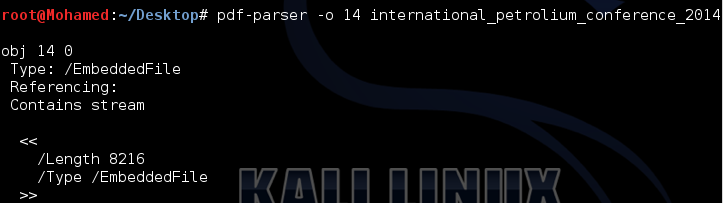
\includegraphics[scale=0.7]{Figures/anal6.png}
\caption{Exemple d'un fichier intégré.}
\label{fig :anal6} 
\end{center}
\end{figure}
\subsection{L'analyse dynamique}
Dans une analyse dynamique nous devons vérifier le fonctionnement global et le fonctionnement interne du code actuellement en l'exécutant dans un environnement contrôlé.  Ceci nous aide à éliminer les faux positifs de la phase d'analyse statique. Des auteurs de malwares incluent du code (techniques d'obfuscation)pour détecter qu'il fonctionne dans les confins d'une machine virtuelle afin de changer son chemin d'exécution.\\

Pour cela on a mis en place un environnements de test s'exécutant
sous MS Windows XP Professional SP3 dans une VirtualBox.\\
Ce document PDF a des techniques "anti-vm", pour les contourner il faut :
\begin{itemize}
\item Arrêter le processus "VBoxService.exe" 
\item Arrêter le processus "VBoxTray.exe"
\item Augmenter la taille de la RAM plus que 512M.
\end{itemize} 
\subsubsection*{Étape 1 : clés de Registres}
On prend un cliché sur l'état de registres avec l'outil "RegShot".
\subsubsection*{Étape 2 : préparation des outils}
\begin{itemize}
\item \textbf{système de fichiers : }définir un filtre pour l'outil "Procmon", on met "category is write"
\item \textbf{Surveiller les processus : }on lance "processus Explorer"
\item \textbf{Surveiller le trafic réseau : }on lance "Wireshark" et "Fakenet".
\end{itemize}
\subsection*{Étape 3 : ouverture du Document PDF} 
double clic sur le document pdf puis on fait :
\begin{itemize}
\item On prend un 2eme cliché sur l'état de registres
\item Arreter les captures dans "Process Monitor" et "Wireshark".
\end{itemize} 
\subsection*{Etape 4 : Interprétation des résultats}

\subsubsection*{Les clés de registre}
On fait la comparaison entre les deux clichés de "Regshot" on voit dans la figure~\ref{fig :anal9} qu'il y'a un changement de 146 clés de registre. 
\begin{figure}[H]
\begin{center}
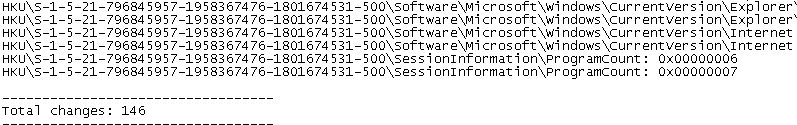
\includegraphics[scale=0.7]{Figures/anal9.png}
\caption{Exemple d'un fichier crée par le document PDF.}
\label{fig :anal9} 
\end{center}
\end{figure}
\subsubsection*{Système de fichiers}
La figure~\ref{fig :anal12} montre que le malware a crée des centaines de fichiers dans le système :
\begin{figure}[H]
\begin{center}
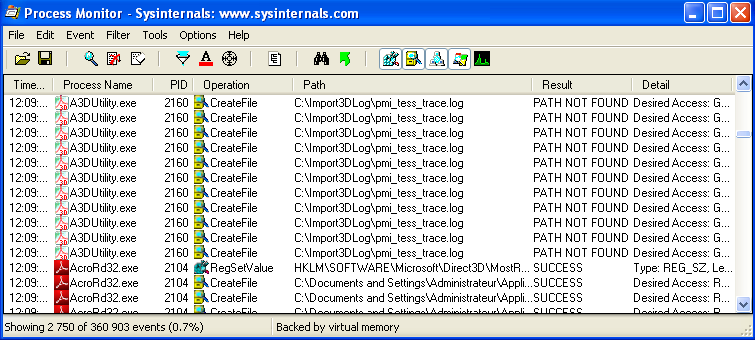
\includegraphics[scale=0.7]{Figures/anal12.png}
\caption{L'interface Processus Monitor.}
\label{fig :anal12} 
\end{center}
\end{figure}
\subsubsection*{Processus suspects}
La figure~\ref{fig :anal7} montre un processus suspect qui a été lancer après l'ouverture du document PDF :
\begin{figure}[H]
\begin{center}
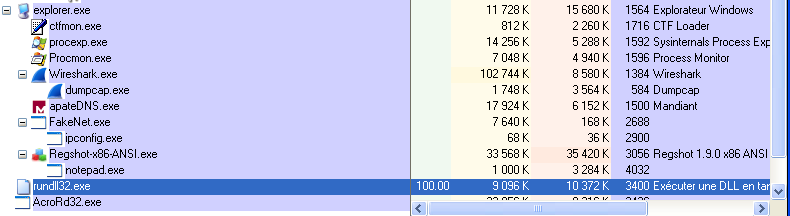
\includegraphics[scale=0.7]{Figures/anal7.png}
\caption{Processus suspect.}
\label{fig :anal7} 
\end{center}
\end{figure}

Après voire les propriétés de ce processus, on voit qu'il a crée un virus "sysinit.ocx" (figure~\ref{fig :anal8})
\begin{figure}[H]
\begin{center}
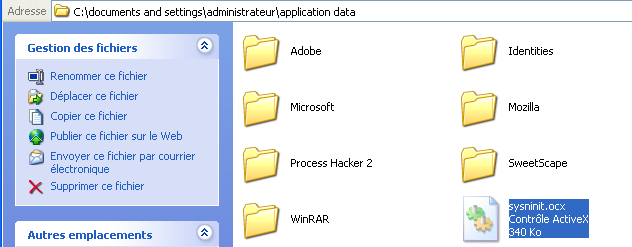
\includegraphics[scale=0.7]{Figures/anal8.png}
\caption{Exemple d'un fichier crée par le document PDF.}
\label{fig :anal8} 
\end{center}
\end{figure}

La figure donne un exemple des fichiers qui se lancent au démarrage de Microsoft Windows :
\begin{figure}[H]
\begin{center}
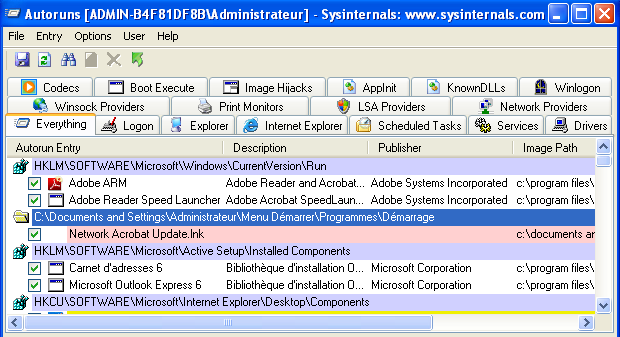
\includegraphics[scale=0.7]{Figures/anal13.png}
\caption{L'interface d'Autoruns.}
\label{fig :anal13} 
\end{center}
\end{figure}
\subsubsection*{Trafic réseau}
Dans la figure on remarque que le malware essaye de contacter le domaine "jhj.wv4.org" et pour tromper la victime que la machine fonctionne bien, il essaye de télécharger les mises à jour de Microsoft Windows.
\begin{figure}[H]
\begin{center}
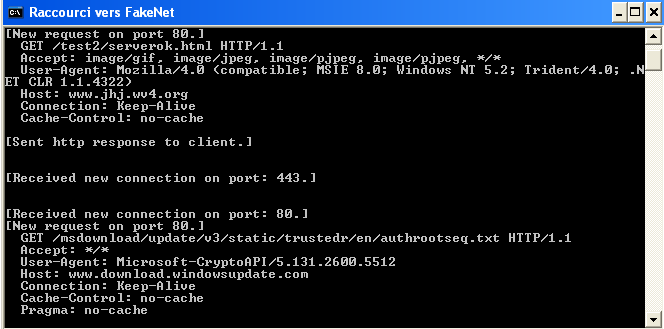
\includegraphics[scale=0.7]{Figures/anal10.png}
\caption{Le trafic réseau par "fakenet".}
\label{fig :anal10} 
\end{center}
\end{figure}
La figure~\ref{fig :anal11} montre que le C\&C server est "jhj.wv4.org" et il essaye de tester si la victime a un accès Internet ou non avec le serveur "google.com".
\begin{figure}[H]
\begin{center}
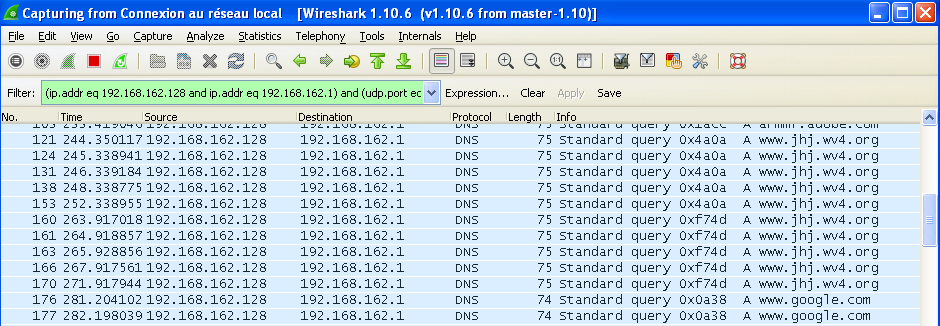
\includegraphics[scale=0.7]{Figures/anal11.png}
\caption{Le trafic réseau par "Wireshark".}
\label{fig :anal11} 
\end{center}
\end{figure}
 
\subsection{Protection contre ce type d'attaques}
Pour se protéger contre ce type d'attaques, il faut mettre à jour Adobe Reader. Et pour la désinfection, il faut supprimer tous les fichiers qui ont été créés par le malware ou d'écrire un script ".bat" qui permet de supprimer les fichiers créés.

\section{Conclusion}

Les malwares sont devenus une réalité pour la majorité des utilisateurs et bien peu d'entre eux y échappent (en particulier sous les systèmes Windows \& Android). Connaître leur mode de fonctionnement ainsi que méthodes de propagation restent le meilleur moyen de s'en protéger. La protection contre les malwares se doit d'être globale et ne peut uniquement se contenter de solutions techniques.\\

Concernant leur analyse, il est possible par l'analyse dynamique d'avoir en quelques minutes les principales caractéristiques d'un malware ainsi que ses fonctionnalités et ce, sans nécessiter de solides connaissances en assembleur. Ce n'est malheureusement pas possible dans certains cas, où les malwares sont capables de détecter les environnements virtuels ou surveillés, et dans ces cas-là, seule une analyse par désassemblage peut permettre d'évaluer la menace.\\

